\documentclass{standalone}
\usepackage{tikz}
\usetikzlibrary{patterns, positioning}


\begin{document}
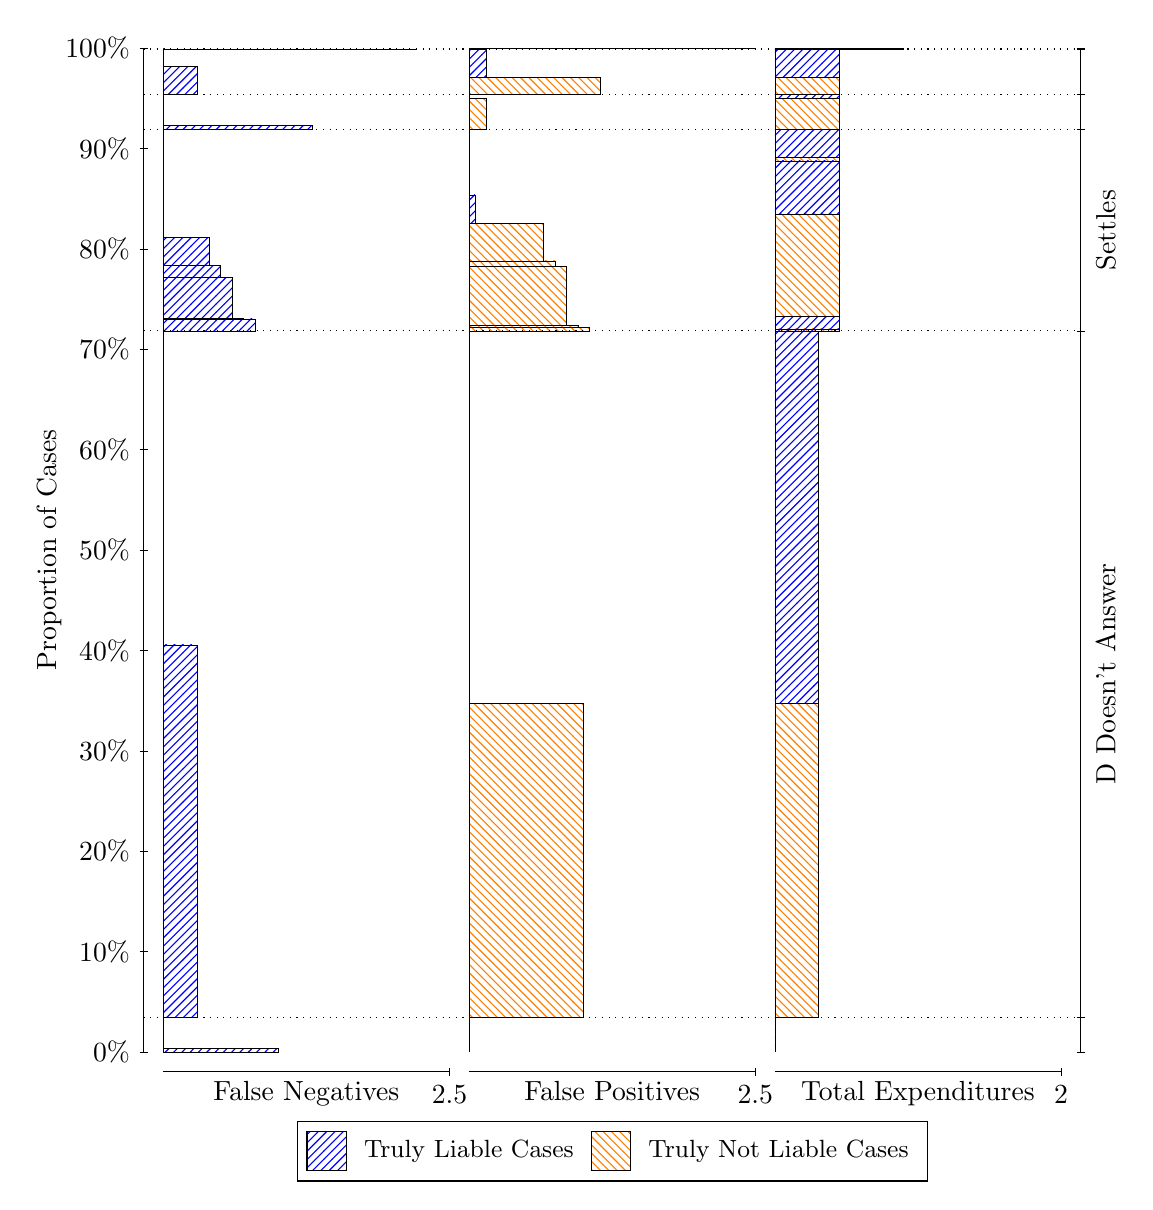
\begin{tikzpicture}
\draw[black, very thin] (1.5,1.75) -- (1.5,14.5);
\node[rotate=90, text=black, anchor=center] at (0.3, 8.125) {Proportion of Cases};
\draw[black, very thin] (1.45,1.75) -- (1.55,1.75);
\node[text=black, anchor=east] at (1.45, 1.75) {0\%};
\draw[black, very thin] (1.45,3.025) -- (1.55,3.025);
\node[text=black, anchor=east] at (1.45, 3.025) {10\%};
\draw[black, very thin] (1.45,4.3) -- (1.55,4.3);
\node[text=black, anchor=east] at (1.45, 4.3) {20\%};
\draw[black, very thin] (1.45,5.575) -- (1.55,5.575);
\node[text=black, anchor=east] at (1.45, 5.575) {30\%};
\draw[black, very thin] (1.45,6.85) -- (1.55,6.85);
\node[text=black, anchor=east] at (1.45, 6.85) {40\%};
\draw[black, very thin] (1.45,8.125) -- (1.55,8.125);
\node[text=black, anchor=east] at (1.45, 8.125) {50\%};
\draw[black, very thin] (1.45,9.4) -- (1.55,9.4);
\node[text=black, anchor=east] at (1.45, 9.4) {60\%};
\draw[black, very thin] (1.45,10.675) -- (1.55,10.675);
\node[text=black, anchor=east] at (1.45, 10.675) {70\%};
\draw[black, very thin] (1.45,11.95) -- (1.55,11.95);
\node[text=black, anchor=east] at (1.45, 11.95) {80\%};
\draw[black, very thin] (1.45,13.225) -- (1.55,13.225);
\node[text=black, anchor=east] at (1.45, 13.225) {90\%};
\draw[black, very thin] (1.45,14.5) -- (1.55,14.5);
\node[text=black, anchor=east] at (1.45, 14.5) {100\%};

\draw[black, very thin] (13.4,1.75) -- (13.4,14.5);
\draw[black, very thin] (13.35,1.75) -- (13.45,1.75);
\node[anchor=west] at (13.35, 1.75) {};
\draw[black, very thin] (13.35,2.1898) -- (13.45,2.1898);
\node[anchor=west] at (13.35, 2.1898) {};
\draw[black, very thin] (13.35,10.909) -- (13.45,10.909);
\node[anchor=west] at (13.35, 10.909) {};
\draw[black, very thin] (13.35,13.469) -- (13.45,13.469);
\node[anchor=west] at (13.35, 13.469) {};
\draw[black, very thin] (13.35,13.912) -- (13.45,13.912);
\node[anchor=west] at (13.35, 13.912) {};
\draw[black, very thin] (13.35,14.482) -- (13.45,14.482);
\node[anchor=west] at (13.35, 14.482) {};
\draw[black, very thin] (13.35,14.494) -- (13.45,14.494);
\node[anchor=west] at (13.35, 14.494) {};
\draw[black, very thin] (13.35,14.5) -- (13.45,14.5);
\node[anchor=west] at (13.35, 14.5) {};

\draw[black, very thin, pattern color=blue, pattern=north east lines] (1.75,1.75) rectangle (3.2033,1.7963);
\draw[black, very thin, pattern color=orange, pattern=north west lines] (1.75,1.7963) rectangle (1.75,2.1898);
\draw[black, very thin, pattern color=blue, pattern=north east lines] (1.75,2.1898) rectangle (2.186,6.9212);
\draw[black, very thin, pattern color=orange, pattern=north west lines] (1.75,6.9212) rectangle (1.75,10.909);
\draw[black, very thin, pattern color=blue, pattern=north east lines] (1.75,10.909) rectangle (2.9127,11.059);
\draw[black, very thin, pattern color=blue, pattern=north east lines] (1.75,11.059) rectangle (2.7673,11.065);
\draw[black, very thin, pattern color=blue, pattern=north east lines] (1.75,11.065) rectangle (2.622,11.583);
\draw[black, very thin, pattern color=blue, pattern=north east lines] (1.75,11.583) rectangle (2.4767,11.744);
\draw[black, very thin, pattern color=blue, pattern=north east lines] (1.75,11.744) rectangle (2.3313,12.1);
\draw[black, very thin, pattern color=orange, pattern=north west lines] (1.75,12.1) rectangle (1.75,13.469);
\draw[black, very thin, pattern color=blue, pattern=north east lines] (1.75,13.469) rectangle (3.6393,13.518);
\draw[black, very thin, pattern color=orange, pattern=north west lines] (1.75,13.518) rectangle (1.75,13.912);
\draw[black, very thin, pattern color=blue, pattern=north east lines] (1.75,13.912) rectangle (2.186,14.263);
\draw[black, very thin, pattern color=orange, pattern=north west lines] (1.75,14.263) rectangle (1.75,14.482);
\draw[black, very thin, pattern color=blue, pattern=north east lines] (1.75,14.482) rectangle (4.9473,14.485);
\draw[black, very thin, pattern color=orange, pattern=north west lines] (1.75,14.485) rectangle (1.75,14.494);
\draw[black, very thin, pattern color=orange, pattern=north west lines] (1.75,14.494) rectangle (1.75,14.497);
\draw[black, very thin, pattern color=blue, pattern=north east lines] (1.75,14.497) rectangle (1.75,14.5);
\draw[black, very thin, pattern color=orange, pattern=north west lines] (5.6333,1.75) rectangle (5.6333,2.1435);
\draw[black, very thin, pattern color=blue, pattern=north east lines] (5.6333,2.1435) rectangle (5.6333,2.1898);
\draw[black, very thin, pattern color=orange, pattern=north west lines] (5.6333,2.1898) rectangle (7.0867,6.1778);
\draw[black, very thin, pattern color=blue, pattern=north east lines] (5.6333,6.1778) rectangle (5.6333,10.909);
\draw[black, very thin, pattern color=orange, pattern=north west lines] (5.6333,10.909) rectangle (7.1593,10.953);
\draw[black, very thin, pattern color=orange, pattern=north west lines] (5.6333,10.953) rectangle (7.014,10.978);
\draw[black, very thin, pattern color=orange, pattern=north west lines] (5.6333,10.978) rectangle (6.8687,11.729);
\draw[black, very thin, pattern color=orange, pattern=north west lines] (5.6333,11.729) rectangle (6.7233,11.797);
\draw[black, very thin, pattern color=orange, pattern=north west lines] (5.6333,11.797) rectangle (6.578,12.277);
\draw[black, very thin, pattern color=blue, pattern=north east lines] (5.6333,12.277) rectangle (5.706,12.634);
\draw[black, very thin, pattern color=blue, pattern=north east lines] (5.6333,12.634) rectangle (5.6333,13.469);
\draw[black, very thin, pattern color=orange, pattern=north west lines] (5.6333,13.469) rectangle (5.8513,13.863);
\draw[black, very thin, pattern color=blue, pattern=north east lines] (5.6333,13.863) rectangle (5.6333,13.912);
\draw[black, very thin, pattern color=orange, pattern=north west lines] (5.6333,13.912) rectangle (7.3047,14.132);
\draw[black, very thin, pattern color=blue, pattern=north east lines] (5.6333,14.132) rectangle (5.8513,14.482);
\draw[black, very thin, pattern color=orange, pattern=north west lines] (5.6333,14.482) rectangle (5.6333,14.491);
\draw[black, very thin, pattern color=blue, pattern=north east lines] (5.6333,14.491) rectangle (5.6333,14.494);
\draw[black, very thin, pattern color=orange, pattern=north west lines] (5.6333,14.494) rectangle (9.2667,14.497);
\draw[black, very thin, pattern color=blue, pattern=north east lines] (5.6333,14.497) rectangle (7.8133,14.5);
\draw[black, very thin, pattern color=orange, pattern=north west lines] (9.5167,1.75) rectangle (9.5167,2.1435);
\draw[black, very thin, pattern color=blue, pattern=north east lines] (9.5167,2.1435) rectangle (9.5167,2.1898);
\draw[black, very thin, pattern color=orange, pattern=north west lines] (9.5167,2.1898) rectangle (10.062,6.1778);
\draw[black, very thin, pattern color=blue, pattern=north east lines] (9.5167,6.1778) rectangle (10.062,10.909);
\draw[black, very thin, pattern color=orange, pattern=north west lines] (9.5167,10.909) rectangle (10.334,10.934);
\draw[black, very thin, pattern color=blue, pattern=north east lines] (9.5167,10.934) rectangle (10.334,11.095);
\draw[black, very thin, pattern color=orange, pattern=north west lines] (9.5167,11.095) rectangle (10.334,12.395);
\draw[black, very thin, pattern color=blue, pattern=north east lines] (9.5167,12.395) rectangle (10.334,13.068);
\draw[black, very thin, pattern color=orange, pattern=north west lines] (9.5167,13.068) rectangle (10.334,13.112);
\draw[black, very thin, pattern color=blue, pattern=north east lines] (9.5167,13.112) rectangle (10.334,13.469);
\draw[black, very thin, pattern color=orange, pattern=north west lines] (9.5167,13.469) rectangle (10.334,13.863);
\draw[black, very thin, pattern color=blue, pattern=north east lines] (9.5167,13.863) rectangle (10.334,13.912);
\draw[black, very thin, pattern color=orange, pattern=north west lines] (9.5167,13.912) rectangle (10.334,14.132);
\draw[black, very thin, pattern color=blue, pattern=north east lines] (9.5167,14.132) rectangle (10.334,14.482);
\draw[black, very thin, pattern color=orange, pattern=north west lines] (9.5167,14.482) rectangle (11.152,14.491);
\draw[black, very thin, pattern color=blue, pattern=north east lines] (9.5167,14.491) rectangle (11.152,14.494);
\draw[black, very thin, pattern color=orange, pattern=north west lines] (9.5167,14.494) rectangle (11.152,14.497);
\draw[black, very thin, pattern color=blue, pattern=north east lines] (9.5167,14.497) rectangle (11.152,14.5);
\draw[black, dotted] (1.5,2.1898) -- (13.4,2.1898);
\draw[black, dotted] (1.5,10.909) -- (13.4,10.909);
\draw[black, dotted] (1.5,13.469) -- (13.4,13.469);
\draw[black, dotted] (1.5,13.912) -- (13.4,13.912);
\draw[black, dotted] (1.5,14.482) -- (13.4,14.482);
\draw[black, dotted] (1.5,14.494) -- (13.4,14.494);
\draw[black, very thin] (1.75,1.5) -- (5.3833,1.5);
\node[text=black, anchor=north] at (3.5667, 1.5) {False Negatives};
\draw[black, very thin] (5.3833,1.45) -- (5.3833,1.55);
\node[text=black, anchor=north] at (5.3833, 1.45) {2.5};

\draw[black, very thin] (5.6333,1.5) -- (9.2667,1.5);
\node[text=black, anchor=north] at (7.45, 1.5) {False Positives};
\draw[black, very thin] (9.2667,1.45) -- (9.2667,1.55);
\node[text=black, anchor=north] at (9.2667, 1.45) {2.5};

\draw[black, very thin] (9.5167,1.5) -- (13.15,1.5);
\node[text=black, anchor=north] at (11.333, 1.5) {Total Expenditures};
\draw[black, very thin] (13.15,1.45) -- (13.15,1.55);
\node[text=black, anchor=north] at (13.15, 1.45) {2};


\node[text=black, centered, rotate=90] at (13.72, 6.5495) {D Doesn't Answer};
\node[text=black, centered, rotate=90] at (13.72, 12.189) {Settles};





\draw (7.449999999999999,1.5) node[draw=none] (baseCoordinate) {};
\begin{scope}[align=center]
        \matrix[scale=0.5, draw=black, below=0.5cm of baseCoordinate, nodes={draw}, column sep=0.1cm]{
            \node[rectangle, draw, minimum width=0.5cm, minimum height=0.5cm, pattern color=blue, pattern=north east lines] {}; &
            \node[draw=none, font=\small, text=black] (B) {Truly Liable Cases}; &
            \node[rectangle, draw, minimum width=0.5cm, minimum height=0.5cm, pattern color=orange, pattern=north west lines] {}; &
            \node[draw=none, font=\small, text=black] (B) {Truly Not Liable Cases}; \\
            };
\end{scope}

\end{tikzpicture}
\end{document}